\documentclass[14pt, usenames,dvipsnames]{beamer} %
% \renewcommand{\baselinestretch}{1.3}
\usepackage[T1]{fontenc}
\usepackage{lmodern}
\usepackage{minted}
\usepackage{xcolor}
\usepackage{etoolbox}
\usepackage{tikz}
\usepackage{color, colortbl}

\usetikzlibrary{mindmap,trees,shadows}
\tikzset{
  invisible/.style={opacity=0},
  visible on/.style={alt={#1{}{invisible}}},
  alt/.code args={<#1>#2#3}{%
    \alt<#1>{\pgfkeysalso{#2}}{\pgfkeysalso{#3}} % \pgfkeysalso doesn't change the path
  },
}


\definecolor{aliceblue}{rgb}{0.94, 0.97, 1.0}
\definecolor{beige}{rgb}{0.96, 0.96, 0.86}
\definecolor{chartreuse}{rgb}{0.87, 1.0, 0.0}

\usemintedstyle{manni}
\setminted{fontsize=\footnotesize, baselinestretch=1}

\setbeamertemplate{footline}[frame number]
\setbeamercolor{normal text}{fg=black!80,bg=white}
\title{Parallel Computing in Python}
\subtitle{Current State and Recent Advances}
\author{\href{http://kbroman.org}{Pierre Glaser}}


\begin{document}
\begin{frame}[fragile]{}
    \titlepage
\end{frame}

\vspace{3em}

\begin{frame}[t]{}
    \center
    \vspace{3em}
    \tableofcontents[
        subsectionstyle=hide/hide/hide,
        sectionstyle=show
        ]
\end{frame}

\section{Python Interfaces with Parallel Computing}
    \subsection{Python? }
    \begin{frame}[t]{Python? What for?}
        \begin{figure}[htpb]
            \vspace*{-0.5cm}
            \hspace*{-1.3cm}
            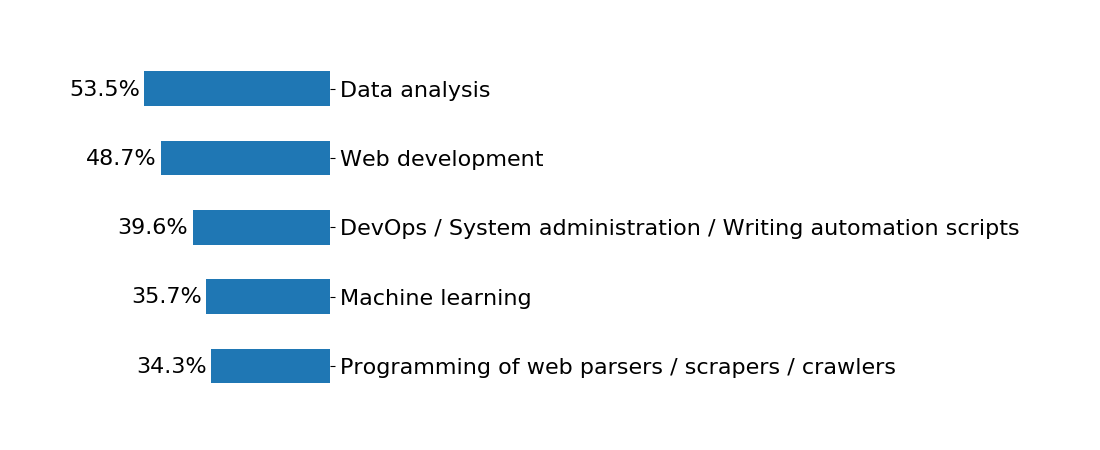
\includegraphics[width=1.1\linewidth]{media/psf_usage_survey.png}
            \vspace*{-0.5cm}
            \caption{\centering{Python usage among developers
        \footnote{\tiny source: https://www.jetbrains.com/research/python-developers-survey-2018/}
            }}
            \label{fig:media/better_screenshot_python_development_results}
        \end{figure}
    \end{frame}
    \begin{frame}{A growing scientific computing ecosystem}
        \begin{tikzpicture}
        \node[align=left] (inst) at (1, 0) {%
        
\includegraphics[scale=0.40]{media/scikit-learn-logo.png}};
        \node[align=left] (inst) at (1, -1) {%
        
\includegraphics[scale=0.4]{media/used_by_scikit-learn.png}};
        \node[align=left] (inst) at (8.5, 0) {%
        
\includegraphics[scale=0.30]{media/numpy-logo.png}};
        \node[align=left] (inst) at (8.5, -1.5) {%
        
\includegraphics[scale=0.4]{media/used_by_numpy.png}};
        \node[align=left] (inst) at (4.5, -3) {%
        
\includegraphics[scale=0.40]{media/pandas.png}};
        \node[align=left] (inst) at (4.5, -4.3) {%
        
\includegraphics[scale=0.4]{media/used_by_pandas.png}};
        \end{tikzpicture}
    \end{frame}
    \begin{frame}[t]{Parallel computing? Why?}
        \small
        \begin{itemize}
            \item going bigger
            \item accelerating repeated experiments
        \end{itemize}
    \end{frame}
    \begin{frame}[t]{Parallel computing? Why?}
        \footnotesize
        \center
        \begin{tikzpicture}
        \node[align=left, visible on=<1>] (all) at (5, 3.5) {%
            \begin{tabular}{c c}
                a & b \\
                \hline
                \hline
                1 & 2 \\
                3 & 4 \\
                5 & 6 \\
                7 & 8 \\
        \end{tabular}};
        \node[align=left, visible on=<2>] (all) at (5, 3.5) {%
            \begin{tabular}{c c}
                a & b \\
                \hline
                \hline
                \rowcolor{beige}
                1 & 2 \\
                3 & 4 \\
                \rowcolor{beige}
                5 & 6 \\
                \rowcolor{beige}
                7 & 8 \\
        \end{tabular}};
        \node[align=left, visible on=<3>] (all) at (5, 3.5) {%
            \begin{tabular}{c c}
                a & b \\
                \hline
                \hline
                1 & 2 \\
                \rowcolor{aliceblue}
                3 & 4 \\
                \rowcolor{aliceblue}
                5 & 6 \\
                \rowcolor{aliceblue}
                7 & 8 \\
        \end{tabular}};
        \node[align=left, visible on=<4->] (all) at (5, 3.5) {%
            \begin{tabular}{c c}
                a & b \\
                \hline
                \hline
                \rowcolor{chartreuse}
                1 & 2 \\
                \rowcolor{chartreuse}
                3 & 4 \\
                \rowcolor{chartreuse}
                5 & 6 \\
                7 & 8 \\
        \end{tabular}};
        \node[align=left, visible on=<2->] (cv1) at (1.5, 0) {%
                \begin{tabular}{c c}
                    a & b \\
                    \hline
                    \hline
                    \rowcolor{beige}
                    1 & 2 \\
                      &   \\
                    \rowcolor{beige}
                    5 & 6 \\
                    \rowcolor{beige}
                    7 & 8 \\
                \end{tabular}};
        \node[align=left, visible on = <3->] (cv2) at (5, 0) {%
            \begin{tabular}{c c}
                a & b \\
                \hline
                \hline
                  &   \\
                \rowcolor{aliceblue}
                3 & 4 \\
                \rowcolor{aliceblue}
                5 & 6 \\
                \rowcolor{aliceblue}
                7 & 8 \\
            \end{tabular}};
        \node[align=left, visible on=<4->] (cv3) at (8.5, 0) {%
                \begin{tabular}{c c}
                    a & b \\
                    \hline
                    \hline
                    \rowcolor{chartreuse}
                    1 & 2 \\
                    \rowcolor{chartreuse}
                    5 & 6 \\
                    \rowcolor{chartreuse}
                    3 & 4 \\
                      &   \\
                \end{tabular}};
        \node[align=left, visible on = <3->] (img) at (8.5, -1.5){%
            \only<6>{
\includegraphics[scale=0.04]{media/server-logo.png}}
            \only<5>{
\includegraphics[scale=0.04]{media/cpu-logo.png}}};
        \node[align=left, visible on = <3->] (img) at (5, -1.5){%
            \only<6>{
\includegraphics[scale=0.04]{media/server-logo.png}}
            \only<5>{
\includegraphics[scale=0.04]{media/cpu-logo.png}}};
        \node[align=left, visible on = <3->] (img) at (1.5, -1.5){%
            \only<6>{
\includegraphics[scale=0.04]{media/server-logo.png}}
            \only<5>{
\includegraphics[scale=0.04]{media/cpu-logo.png}}};
        {\draw[->, visible on=<2->] (all.south)--(cv1.north east);}
        {\draw[->, visible on=<3->] (all.south)--(cv2.north);}
        {\draw[->, visible on=<4->] (all.south)--(cv3.north west);}
        \end{tikzpicture}
    \end{frame}
    \begin{frame}[t]{}
        \center
        \vspace{3em}
        \tableofcontents[
            % currentsubsection,
            % hideothersubsections,
            subsectionstyle=show/hide/hide,
            sectionstyle=show/hide
            ]
    \end{frame}
    \begin{frame}[t]{Our concerns}
        \centering{communication}
        \small
        \begin{itemize}
            \item speed
            \item safety (deadlocks)
            \item memory footprint
        \end{itemize}
    \end{frame}
    \begin{frame}[t]{}
        \vspace{5em}
        \center Disclaimer: This talk is mostly CPython specific.
    \end{frame}

    % \subsection{At which level?}
    %     \begin{frame}[t]{The Python Interpreter}

    %     \end{frame}
    %     \begin{frame}[t]{Parallelism at the Python level}

    %     \end{frame}
    %     \begin{frame}[t]{Parallelism at the C level}
    %     \end{frame}
    % \subsection{Using which code?}
    %     \begin{frame}[t]{The python virtual machine}

    %     \end{frame}
    %     \begin{frame}[t]{Arbirtray code execution}

    %     \end{frame}
    %     \begin{frame}[t]{Consequences for paralle computing}

    %     \end{frame}
    % \subsection{In practice?}
    %     \begin{frame}[t]{several matrix-matrix multiplication}
    %         \begin{itemize}
    %             \item using python threads
    %             \item using python processes
    %             \item using BLAS parallelism
    %         \end{itemize}
    %     \end{frame}



\section{Built-in and Third Party ressources}
    \subsection{In the Standard Library}
        \begin{frame}[t]{multiprocessing}

        \end{frame}
        \begin{frame}[t]{concurrent futures}

        \end{frame}
    \subsection{Third party extensions}
        \begin{frame}[t]{loky}

        \end{frame}
        \begin{frame}[t]{joblib}

        \end{frame}
    \subsection{From one to another}
        \begin{frame}[t]{going upstream}

        \end{frame}

\section{Recent Advances}
\subsection{Why we need better IPC}
\subsection{Better extensibility of the pickle module}
\subsection{PEP 574}
    \begin{frame}[t]{principle}
    \end{frame}

    \begin{frame}[t]{better memory footrpint}
    \end{frame}

    \begin{frame}[t]{better speed}
    \end{frame}
\subsection{built-in shared memory in the standard library}



\begin{frame}[fragile]{}
    \setbeamercolor{block body}{bg=beige}
    \begin{beamerboxesrounded}{}
        \inputminted[fontfamily=fvm, bgcolor=beige]{python}{scripts/test_script.py}
    \end{beamerboxesrounded}
\end{frame}
\end{document}
